\makeatletter
\tikzset{
    database/.style={
        path picture={
            \draw (0, 1.5*\database@segmentheight) circle [x radius=\database@radius,y radius=\database@aspectratio*\database@radius];
            \draw (-\database@radius, 0.5*\database@segmentheight) arc [start angle=180,end angle=360,x radius=\database@radius, y radius=\database@aspectratio*\database@radius];
            \draw (-\database@radius,-0.5*\database@segmentheight) arc [start angle=180,end angle=360,x radius=\database@radius, y radius=\database@aspectratio*\database@radius];
            \draw (-\database@radius,1.5*\database@segmentheight) -- ++(0,-3*\database@segmentheight) arc [start angle=180,end angle=360,x radius=\database@radius, y radius=\database@aspectratio*\database@radius] -- ++(0,3*\database@segmentheight);
        },
        minimum width=2*\database@radius + \pgflinewidth,
        minimum height=3*\database@segmentheight + 2*\database@aspectratio*\database@radius + \pgflinewidth,
    },
    database segment height/.store in=\database@segmentheight,
    database radius/.store in=\database@radius,
    database aspect ratio/.store in=\database@aspectratio,
    database segment height=0.1cm,
    database radius=0.25cm,
    database aspect ratio=0.35,
}
\makeatother


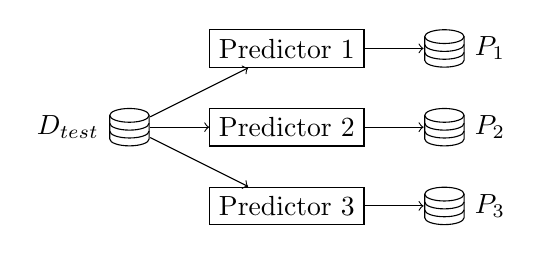
\begin{tikzpicture}
\node[database,label=left:$D_{\text{test}}$] (test) at (0,-1){};

\node[rectangle,draw] (pred1) at (2,0) {Predictor 1};
\node[rectangle,draw] (pred2) at (2,-1) {Predictor 2};
\node[rectangle,draw] (pred3) at (2,-2) {Predictor 3};


\node[database,label=right:$P_{1}$] (p1) at (4,0){};
\node[database,label=right:$P_{2}$] (p2) at (4,-1){};
\node[database,label=right:$P_{3}$] (p3) at (4,-2){};

\draw[->] (test) to (pred1);
\draw[->] (test) to (pred2);
\draw[->] (test) to (pred3);

\draw[->] (pred1) to (p1);
\draw[->] (pred2) to (p2);
\draw[->] (pred3) to (p3);

\end{tikzpicture}
